\section{Robot Design}
% describe the design
% what are the advantages
We mainly focus on two aspects when configuring the Lego robot, namely {\itshape \rom{1})} stability and {\itshape \rom{2})} feasibility. The complete configuration of the robot is visualised in Fig.\ref{fig:robotconfig}, where there are three images showing the front, side and back appearances of the robot respectively. 

The total height of the robot is approximately 18 cm. The width and length are 13 cm and 19.5 cm, respectively. This configuration ensures that the robot does not occupy too much space in the arena. The ultrasonic sensor is placed in the lower front with an approximate height of 6.5 cm and has a vision range of 180 degrees. A previous prototype with the sensor on the top and 360 degrees of freedom was tested but the wire connected to de brick interfered the sensor spin. A novel feature used in this design is the support device installed in the back as shown in Fig.\ref{fig:backrobot}, where two balls are positioned inside the two white slots to reduce the friction between the ground and the support device while rotating and moving. 

\begin{figure}[h]
\centering
  \begin{subfigure}{0.25\textwidth}
  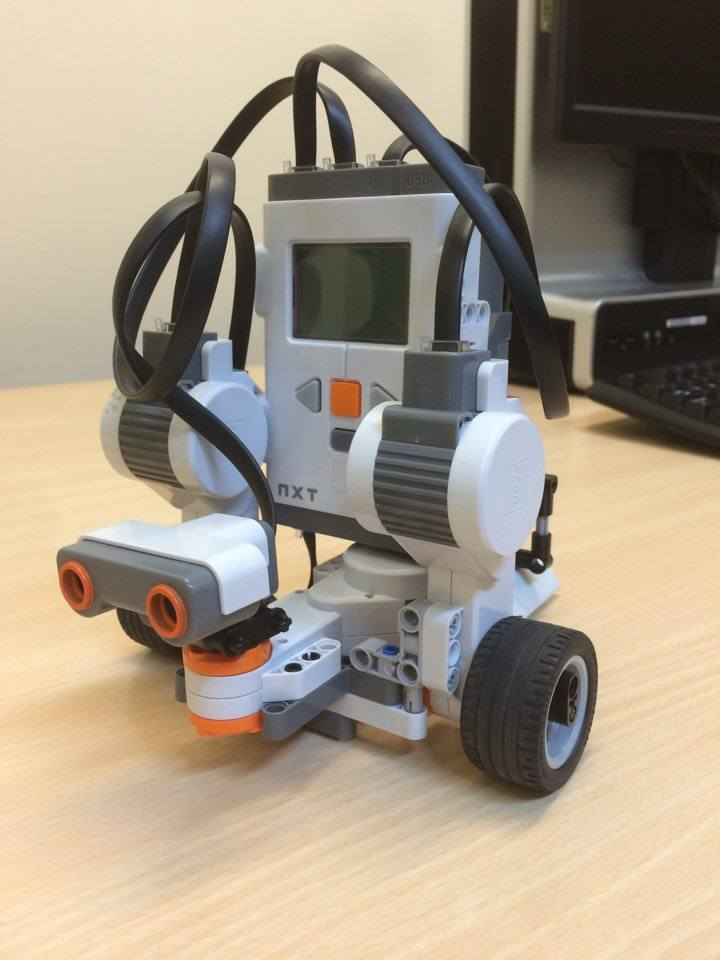
\includegraphics[scale=0.15]{f}
  \caption{Front appearance}
  \end{subfigure}
  \begin{subfigure}{0.25\textwidth}
  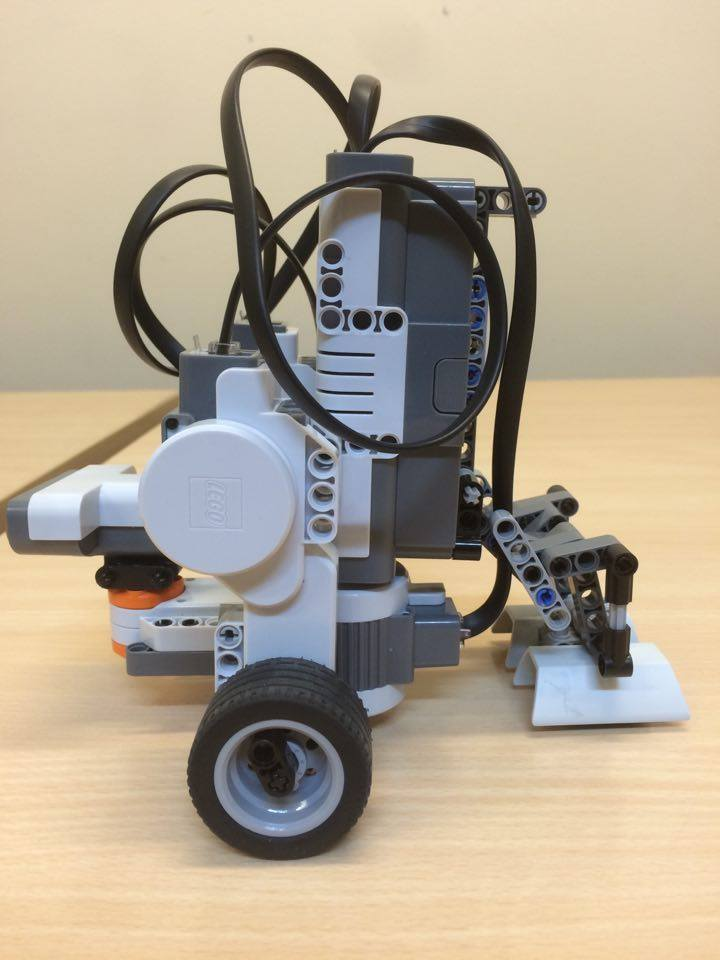
\includegraphics[scale=0.15]{s}
  \caption{Side appearance}
  \end{subfigure}
  \begin{subfigure}{0.25\textwidth}
  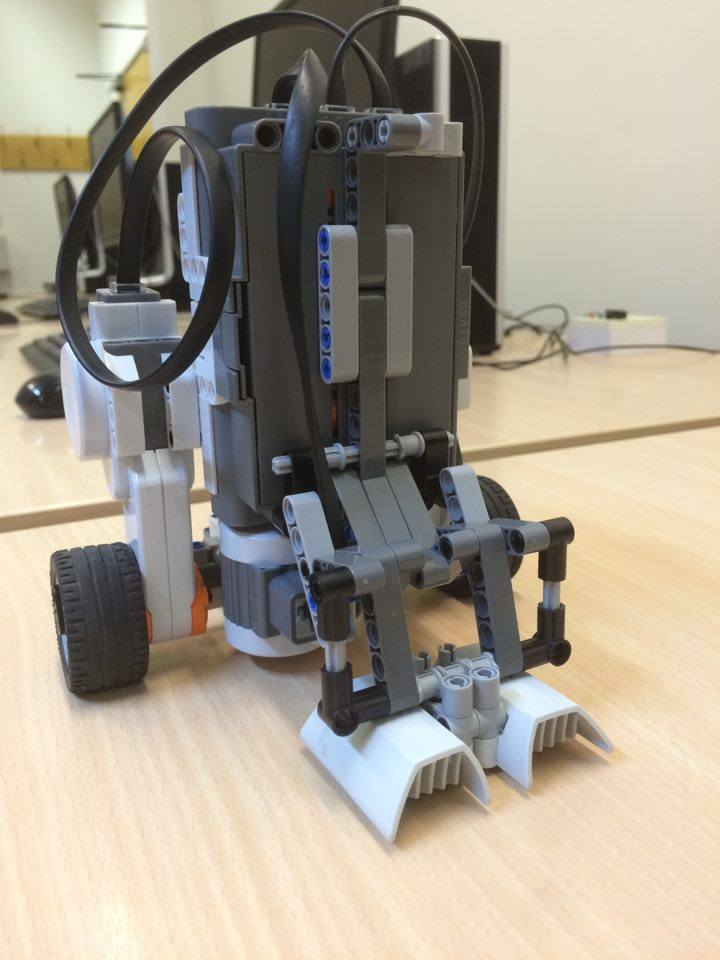
\includegraphics[scale=0.15]{b}
  \caption{Back appearance} \label{fig:backrobot}
  \end{subfigure}
  \caption{Robot configuration.}
  \label{fig:robotconfig}
\end{figure}

\FloatBarrier
